% Options for packages loaded elsewhere
% Options for packages loaded elsewhere
\PassOptionsToPackage{unicode}{hyperref}
\PassOptionsToPackage{hyphens}{url}
\PassOptionsToPackage{dvipsnames,svgnames,x11names}{xcolor}
%
\documentclass[
  letterpaper,
  DIV=11,
  numbers=noendperiod]{scrartcl}
\usepackage{xcolor}
\usepackage{amsmath,amssymb}
\setcounter{secnumdepth}{5}
\usepackage{iftex}
\ifPDFTeX
  \usepackage[T1]{fontenc}
  \usepackage[utf8]{inputenc}
  \usepackage{textcomp} % provide euro and other symbols
\else % if luatex or xetex
  \usepackage{unicode-math} % this also loads fontspec
  \defaultfontfeatures{Scale=MatchLowercase}
  \defaultfontfeatures[\rmfamily]{Ligatures=TeX,Scale=1}
\fi
\usepackage{lmodern}
\ifPDFTeX\else
  % xetex/luatex font selection
\fi
% Use upquote if available, for straight quotes in verbatim environments
\IfFileExists{upquote.sty}{\usepackage{upquote}}{}
\IfFileExists{microtype.sty}{% use microtype if available
  \usepackage[]{microtype}
  \UseMicrotypeSet[protrusion]{basicmath} % disable protrusion for tt fonts
}{}
\makeatletter
\@ifundefined{KOMAClassName}{% if non-KOMA class
  \IfFileExists{parskip.sty}{%
    \usepackage{parskip}
  }{% else
    \setlength{\parindent}{0pt}
    \setlength{\parskip}{6pt plus 2pt minus 1pt}}
}{% if KOMA class
  \KOMAoptions{parskip=half}}
\makeatother
% Make \paragraph and \subparagraph free-standing
\makeatletter
\ifx\paragraph\undefined\else
  \let\oldparagraph\paragraph
  \renewcommand{\paragraph}{
    \@ifstar
      \xxxParagraphStar
      \xxxParagraphNoStar
  }
  \newcommand{\xxxParagraphStar}[1]{\oldparagraph*{#1}\mbox{}}
  \newcommand{\xxxParagraphNoStar}[1]{\oldparagraph{#1}\mbox{}}
\fi
\ifx\subparagraph\undefined\else
  \let\oldsubparagraph\subparagraph
  \renewcommand{\subparagraph}{
    \@ifstar
      \xxxSubParagraphStar
      \xxxSubParagraphNoStar
  }
  \newcommand{\xxxSubParagraphStar}[1]{\oldsubparagraph*{#1}\mbox{}}
  \newcommand{\xxxSubParagraphNoStar}[1]{\oldsubparagraph{#1}\mbox{}}
\fi
\makeatother


\usepackage{longtable,booktabs,array}
\usepackage{calc} % for calculating minipage widths
% Correct order of tables after \paragraph or \subparagraph
\usepackage{etoolbox}
\makeatletter
\patchcmd\longtable{\par}{\if@noskipsec\mbox{}\fi\par}{}{}
\makeatother
% Allow footnotes in longtable head/foot
\IfFileExists{footnotehyper.sty}{\usepackage{footnotehyper}}{\usepackage{footnote}}
\makesavenoteenv{longtable}
\usepackage{graphicx}
\makeatletter
\newsavebox\pandoc@box
\newcommand*\pandocbounded[1]{% scales image to fit in text height/width
  \sbox\pandoc@box{#1}%
  \Gscale@div\@tempa{\textheight}{\dimexpr\ht\pandoc@box+\dp\pandoc@box\relax}%
  \Gscale@div\@tempb{\linewidth}{\wd\pandoc@box}%
  \ifdim\@tempb\p@<\@tempa\p@\let\@tempa\@tempb\fi% select the smaller of both
  \ifdim\@tempa\p@<\p@\scalebox{\@tempa}{\usebox\pandoc@box}%
  \else\usebox{\pandoc@box}%
  \fi%
}
% Set default figure placement to htbp
\def\fps@figure{htbp}
\makeatother


% definitions for citeproc citations
\NewDocumentCommand\citeproctext{}{}
\NewDocumentCommand\citeproc{mm}{%
  \begingroup\def\citeproctext{#2}\cite{#1}\endgroup}
\makeatletter
 % allow citations to break across lines
 \let\@cite@ofmt\@firstofone
 % avoid brackets around text for \cite:
 \def\@biblabel#1{}
 \def\@cite#1#2{{#1\if@tempswa , #2\fi}}
\makeatother
\newlength{\cslhangindent}
\setlength{\cslhangindent}{1.5em}
\newlength{\csllabelwidth}
\setlength{\csllabelwidth}{3em}
\newenvironment{CSLReferences}[2] % #1 hanging-indent, #2 entry-spacing
 {\begin{list}{}{%
  \setlength{\itemindent}{0pt}
  \setlength{\leftmargin}{0pt}
  \setlength{\parsep}{0pt}
  % turn on hanging indent if param 1 is 1
  \ifodd #1
   \setlength{\leftmargin}{\cslhangindent}
   \setlength{\itemindent}{-1\cslhangindent}
  \fi
  % set entry spacing
  \setlength{\itemsep}{#2\baselineskip}}}
 {\end{list}}
\usepackage{calc}
\newcommand{\CSLBlock}[1]{\hfill\break\parbox[t]{\linewidth}{\strut\ignorespaces#1\strut}}
\newcommand{\CSLLeftMargin}[1]{\parbox[t]{\csllabelwidth}{\strut#1\strut}}
\newcommand{\CSLRightInline}[1]{\parbox[t]{\linewidth - \csllabelwidth}{\strut#1\strut}}
\newcommand{\CSLIndent}[1]{\hspace{\cslhangindent}#1}



\setlength{\emergencystretch}{3em} % prevent overfull lines

\providecommand{\tightlist}{%
  \setlength{\itemsep}{0pt}\setlength{\parskip}{0pt}}



 


\KOMAoption{captions}{tableheading}
\makeatletter
\@ifpackageloaded{caption}{}{\usepackage{caption}}
\AtBeginDocument{%
\ifdefined\contentsname
  \renewcommand*\contentsname{Table of contents}
\else
  \newcommand\contentsname{Table of contents}
\fi
\ifdefined\listfigurename
  \renewcommand*\listfigurename{List of Figures}
\else
  \newcommand\listfigurename{List of Figures}
\fi
\ifdefined\listtablename
  \renewcommand*\listtablename{List of Tables}
\else
  \newcommand\listtablename{List of Tables}
\fi
\ifdefined\figurename
  \renewcommand*\figurename{Figure}
\else
  \newcommand\figurename{Figure}
\fi
\ifdefined\tablename
  \renewcommand*\tablename{Table}
\else
  \newcommand\tablename{Table}
\fi
}
\@ifpackageloaded{float}{}{\usepackage{float}}
\floatstyle{ruled}
\@ifundefined{c@chapter}{\newfloat{codelisting}{h}{lop}}{\newfloat{codelisting}{h}{lop}[chapter]}
\floatname{codelisting}{Listing}
\newcommand*\listoflistings{\listof{codelisting}{List of Listings}}
\makeatother
\makeatletter
\makeatother
\makeatletter
\@ifpackageloaded{caption}{}{\usepackage{caption}}
\@ifpackageloaded{subcaption}{}{\usepackage{subcaption}}
\makeatother
\usepackage{bookmark}
\IfFileExists{xurl.sty}{\usepackage{xurl}}{} % add URL line breaks if available
\urlstyle{same}
\hypersetup{
  pdftitle={Regional growth, convergence, and spatial spillovers in India:},
  pdfauthor={Carlos Mendez; Sujana Kabiraj; Jiaqi Li},
  pdfkeywords={Reproducible research, Nighttime lights, Regional
convergence, Spatial spillovers, Spatial Durbin model, India},
  colorlinks=true,
  linkcolor={blue},
  filecolor={Maroon},
  citecolor={Blue},
  urlcolor={Blue},
  pdfcreator={LaTeX via pandoc}}


\title{Regional growth, convergence, and spatial spillovers in India:}
\usepackage{etoolbox}
\makeatletter
\providecommand{\subtitle}[1]{% add subtitle to \maketitle
  \apptocmd{\@title}{\par {\large #1 \par}}{}{}
}
\makeatother
\subtitle{A reproducible view from outer space}
\author{Carlos Mendez \and Sujana Kabiraj \and Jiaqi Li}
\date{}
\begin{document}
\maketitle
\begin{abstract}
Using satellite nighttime light data as proxy for economic activity,
Chanda and Kabiraj (2020, World Development) studied regional growth and
convergence across 520 districts in India. Based on a reproducible
open-science approach, this article builds on their work by confirming
and extending their main findings in three fronts. First, we illustrate
regional convergence patterns using an interactive web-based tool for
satellite image visualization. Second, we assess the degree of spatial
dependence in their main econometric specification. Third, we employ a
spatial Durbin model to measure the role of spatial spillovers in the
convergence process. Our results indicate that spatial spillovers
significantly increase the speed of regional convergence. Overall, the
results emphasize the role of spatial dependence in regional convergence
through the lens of satellite imagery, interactive visualizations, and
spillover modeling.
\end{abstract}


\section{Introduction}\label{introduction}

Regional economic growth and convergence are key concerns in developing
countries, particularly in large federal states like India where spatial
inequalities can threaten social cohesion and political stability.
However, studying regional convergence patterns in developing countries
has been historically challenging due to limited availability of
consistent economic data at subnational administrative levels. The
emergence of satellite nighttime light data as a proxy for economic
activity has created new opportunities to analyze regional growth
dynamics at granular geographic scales.

In an important contribution, Chanda and Kabiraj (2020) leveraged
nighttime light data to document evidence of regional convergence across
520 districts in India between 1996 and 2010. Their analysis showed that
poorer districts grew faster than richer ones during this period,
suggesting a gradual reduction in spatial inequalities. However, their
econometric approach did not account for potential spatial spillovers in
the convergence process---the possibility that a district's growth
trajectory might be influenced not only by its own initial conditions
but also by those of its neighbors.

In this context, this paper confirms and extends the study of Chanda and
Kabiraj (2020) in three key methodological directions. First, we develop
an interactive web-based visualization tool that allows researchers to
dynamically explore spatial and temporal patterns in the nighttime light
data. This tool facilitates the identification of converging regions and
growth hotspots that may be difficult to detect in static
representations. Second, we formally test for spatial dependence in both
the dependent and independent variables of the convergence equations,
highlighting that spatial autocorrelation is an inherent feature of
satellite data and the regional convergence process. Third, we employ a
spatial Durbin model that explicitly accounts for spatial spillovers,
quantifying how neighborhood effects influence the speed of regional
convergence.

Our results yield three main findings that advance our understanding of
regional convergence in India. First, interactive visualization tools
reveal clear spatial patterns in both the initial distribution and
subsequent growth of nighttime lights. Second, formal tests of spatial
dependence indicate that district-level economic trajectories are not
independent of their neighbors. Third, accounting for spatial spillovers
through the spatial Durbin model shows that the total convergence effect
is substantially larger than previous non-spatial estimates would
suggest. Specifically, spatial spillovers appear to accelerate the
convergence process by creating additional channels through which
lagging regions can catch up.

These findings have important implications for both research methodology
and policy design. Methodologically, they demonstrate that conventional
non-spatial approaches may significantly underestimate the speed of
regional convergence by failing to account for inter-district
spillovers. From a policy perspective, they suggest that the benefits of
place-based development interventions may extend beyond target districts
through spatial multiplier effects, potentially increasing their
cost-effectiveness. The results also highlight the value of new data
sources and methodological tools in advancing our understanding of
regional economic dynamics in developing countries.

The rest of this article is organized as follows. Section 2 provides an
overview of the data and methods, describing our use of nighttime light
data as a proxy for economic activity and introducing the spatial Durbin
model that forms the basis of our empirical strategy. We also detail our
methodological extensions related to interactive visualizations, spatial
dependence testing, and spillover modeling. Section 3 presents our
empirical results, beginning with an interactive exploration of regional
convergence patterns, followed by formal tests of spatial dependence,
and concluding with estimates of direct and indirect convergence effects
from the spatial Durbin model. Finally, Section 4 offers some concluding
remarks.

\section{Data and methods}\label{data-and-methods}

\subsection{Data: Nightlights as a proxy for economic
activity}\label{data-nightlights-as-a-proxy-for-economic-activity}

One of the key challenges in studying economic growth in developing
countries like India is the limited availability and reliability of data
on aggregate economic activity at finer administrative levels beyond the
state level. To address this issue, a growing body of literature,
pioneered by Henderson, Storeygard, and Weil (2012), has utilized
satellite nighttime light data as a proxy for economic activity at
sub-national levels.

Nightlight data has been widely used to investigate economic growth and
convergence across national and sub-national regions in various
countries. For instance, Adhikari and Dhital (2020) examine the impact
of decentralization on regional convergence using nightlight data, while
Pinkovskiy and Sala-i-Martin (2016) use nightlight data to adjudicate
between national accounts and household surveys, finding that national
accounts better capture aggregate economic growth. Similarly, Lessmann
and Seidel (2017) leverage nightlight data to estimate GDP per capita
and income inequality globally. More broadly, Gennaioli et al. (2014)
study regional convergence using per capita income data from 1,528
subnational regions across 83 countries, finding a convergence rate of
about 2\% per year.

Nightlight data has been widely utilized in India across various
contexts. For example, Cook and Shah (2022) use nightlight data to
analyze the impact of public welfare programs, while Jha and Talathi
(2021) examine the effects of colonial institutions, and Chanda and Cook
(2022) investigate the impact of demonetization. Beyer, Jain, and Sinha
(2021) employ nightlight data to study the effects of COVID-19. In the
context of convergence studies, Chakravarty and Dehejia (2019) document
significant regional disparities in India using nightlight data and
caution that GST may further exacerbate them, while (Chanda and Kabiraj
2020) highlights district-level convergence.

Our study draws inspiration from (Chanda and Kabiraj 2020). Following
their approach, we use the per capita growth in nightlights as the
dependent variable and the initial nightlights per capita as the primary
variable of interest. These variables are derived from nightlight data
released by the National Geophysical Data Center (NGDC), based on
observations from the DMSP/OLS satellites spanning the period from 1996
to 2010. To mitigate the issue of top-coding in light data, the NGDC
released ``radiance-calibrated'' nighttime lights for eight specific
years within this period. This dataset employs high magnification
settings for low-light regions and low magnification settings for
brightly lit areas. For this study, we utilize the
``radiance-calibrated'' nighttime lights data.\footnote{Following Chanda
  and Kabiraj (2020), our sample consists of 520 districts (out of a
  possible 593). There were 593 districts in 2001, which rose to 640
  districts in the 2011 census. To match the districts among two census
  files, we summed up the curved-out districts with their origin
  districts in the 2011 census files. Eight districts among 47 new
  districts were created by curving out some areas from multiple
  districts. Those new districts along with their multiple-origin
  districts were dropped from our sample. We dropped all the districts
  in the state of Assam where more than 50\% of districts were created
  in that manner.}

\subsection{Modeling regional
convergence}\label{modeling-regional-convergence}

In neoclassical growth models, such as the Solow model, it is argued
that the per capita growth rate should be negatively correlated with a
region's initial endowment primarily due to diminishing returns to
capital. Specifically, poorer regions, assuming similar technology and
preferences, are expected to experience higher growth rates compared to
their wealthier counterparts. Consequently, over the long run, regions
with similar characteristics should converge to a common steady state.
We would like to explore such convergence (denoted by
\textbf{\(\beta\)-convergence}) employing a Barro-style growth
regressions framework. Equation (1) analyzes absolute convergence.

\begin{equation}\phantomsection\label{eq-matrix-form-abs}{
\boldsymbol{g_t} =  \beta_1 \boldsymbol{x_{t-1}} +  \boldsymbol{\varepsilon_t}
}\end{equation}

where \(\boldsymbol{g_t}\) represents an \(N\text{-by-}1\) vector of
observations on NTL growth for each of the \(N\) regions over the period
\(t\) and \(\boldsymbol{x_{t-1}}\) represents an \(N\text{-by-}1\)
vector of observations on the initial (log) level of NTL. The scalar
\(\beta_1\) is a regression coefficient that indicates the direction and
strength of regional convergence. Finally,
\(\boldsymbol{\varepsilon_t}\) represents a vector of idiosyncratic
error terms.

While absolute convergence implies that districts converge to a common
steady state, regions may differ in various aspects such as geography,
socio-economic conditions, and policy implementation. To account for
these differences, we include state dummies in our analysis to examine
whether heterogeneity in state-specific institutions and policies
influences the rate of convergence. Additionally, we control for the
initial share of unlit pixels in districts to address any potential
under-coding in nightlights data.

To further explore the determinants of district-level growth rates, we
incorporate a range of geo-climatic controls alongside initial
district-specific conditions related to demographics, human capital, and
infrastructure. Equation~\ref{eq-matrix-form-abs} explores conditional
convergence.

\begin{equation}\phantomsection\label{eq-matrix-form-cond}{
\boldsymbol{g_t} =  \beta_1 \boldsymbol{x_{t-1}} + \boldsymbol{X_t} \boldsymbol{\alpha}  + \boldsymbol{\varepsilon_t}
}\end{equation}

Here, the matrix \(\boldsymbol{X_t}\) is a \(N\text{-by-}k\) collection
of observations on control variables for each region. The vector
\(\boldsymbol{\alpha}\), with dimensions \(k \times 1\), captures the
regression coefficients for these variables. The control variables are
listed in Table A.1 in Chanda and Kabiraj (2020).

\subsection{Interactive spatial
visualizations}\label{interactive-spatial-visualizations}

Interactive visualizations of nighttime lights imagery offer distinct
methodological advantages over static representations, particularly when
analyzing temporal and spatial heterogeneity in economic activity. The
dynamic nature of these visualizations enables researchers to
simultaneously examine multiple dimensions of the data, including
temporal variations in light intensity, the spatial distribution of
economic activity, and the relationship between nighttime lights and
other georeferenced variables. This interactivity is especially valuable
when investigating economic phenomena that exhibit significant spatial
and temporal variation, such as urbanization patterns, economic shocks,
or regional development disparities. The ability to dynamically adjust
visualization parameters, such as temporal ranges, spatial scales, and
light intensity thresholds, allows for more nuanced exploration of
economic patterns that might be obscured in static representations.

Google Earth Engine (GEE) substantially reduces the computational and
technical barriers to creating such interactive visualizations, offering
a particularly advantageous platform for economic research utilizing
nighttime lights data. The platform's browser-based integrated
development environment facilitates the creation of interactive web
applications without requiring extensive infrastructure or specialized
software installation. This capability is especially valuable for
reproducible research, as it enables the development of web applications
that can be shared with other researchers or stakeholders, allowing them
to interact with the data and verify findings independently. The
platform's ability to handle large-scale geospatial computations
server-side, combined with its extensive catalog of pre-processed
nighttime lights datasets, including the DMSP-OLS and VIIRS collections,
significantly streamlines the workflow from raw data to interactive
visualization. This computational efficiency is particularly beneficial
when analyzing long time series or large geographic areas, which would
be computationally intensive using traditional desktop-based approaches.

Interactive visualizations of nighttime lights data are particularly
instrumental in identifying and analyzing patterns of regional
convergence in luminosity, providing visual insights into economic
convergence processes. Through dynamic visualization tools, researchers
can track the evolution of light intensity across regions over time,
effectively identifying areas that exhibit catch-up growth patterns -
where initially dim regions progressively converge toward the luminosity
levels of their brighter counterparts.

\subsection{Spatial dependence
testing}\label{spatial-dependence-testing}

The analysis of regional convergence using nighttime light data requires
explicit consideration of spatial dependence patterns across Indian
districts. To formally test and account for such spatial relationships,
we employ the global Moran's I test and applied to the main variables of
the convergence Equation~\ref{eq-matrix-form-cond} . The Moran's I test
quantifies the degree of spatial autocorrelation among geographic units
and can be expressed as:

\[
I=\frac{\sum_i \Sigma_j w_{i j} z_i \cdot z_j /\sum_i \Sigma_j w_{i j}}{\Sigma_i z_i^2 / n}
\] where \(z_i\) represents the deviation of observation \(i\) from the
mean, and \(w_{ij}\) denotes the spatial weight between units \(i\) and
\(j\). The Moran statistic can range from -1 to +1, with positive values
indicating spatial clustering and negative values suggesting spatial
dispersion.

The specification of the spatial weights matrix \(\mathbf{W}\) is
crucial for capturing the underlying spatial structure. We primarily
employ a Queen contiguity matrix defined as:

\[
\mathbf{W}=\left[\begin{array}{ccccc}
w_{11} & w_{12} & w_{13} & \cdots & w_{1 \mathrm{n}} \\
w_{21} & w_{22} & w_{23} & \cdots & w_{2 \mathrm{n}} \\
\vdots & \vdots & \vdots & w_{\mathrm{ij}} & \vdots \\
w_{\mathrm{n} 1} & w_{\mathrm{n} 2} & w_{\mathrm{n} 3} & \cdots & w_{\mathrm{nn}}
\end{array}\right]
\] where \(w_{ij}=1\) for districts sharing either a border or vertex
and 0 otherwise. Following standard practice, we row-normalize the
weights matrix.

The detection of significant spatial dependence would justify the use of
spatial econometric techniques. In particular, Ertur and Koch (2007) and
Fischer (2011) argue that the spatial Durbin model can properly account
for spatial spillovers in the convergence process. This methodological
choice allows us to distinguish between direct effects of district
characteristics and indirect effects operating through spatial channels.

\subsection{Spatial spillover
modeling}\label{spatial-spillover-modeling}

Our spatial spillover modeling builds upon the spatial Solow growth
model developed by Ertur and Koch (2007) and Fischer (2011), which
extends the traditional Solow framework to account for technological
interdependence across regions. The model considers an economy of \(N\)
subnational regions, each characterized by a Cobb-Douglas production
function with constant returns to scale:

\begin{equation}\phantomsection\label{eq-production}{
Y_{i t}=A_{i t} K_{i t}^{\alpha_{K}} H_{i t}^{\alpha_{H}} L_{i t}^{1-\alpha_{K} -\alpha_{H}}
}\end{equation}

where \(Y_{it}\) represents output, \(K_{it}\) physical capital,
\(H_{it}\) human capital, \(L_{it}\) labor force, and \(A_{it}\) the
level of technological knowledge for region \(i\) at time \(t\). The
parameters \(\alpha_K\) and \(\alpha_H\) denote the output elasticities
with respect to physical and human capital, respectively. A key
innovation of this framework is the modeling of technological knowledge,
which incorporates both internal and external factors:

\begin{equation}\phantomsection\label{eq-technology}{
A_{i t}=\Omega_{t} k_{i t}^{\theta} h_{i t}^{\phi} \prod_{j \neq i}^{N} A_{j t}^{\rho W_{i j}}
}\end{equation}

This specification captures three distinct components of technological
progress:

\begin{itemize}
\tightlist
\item
  An exogenous component (\(\Omega_t\)) representing the common stock of
  knowledge across regions
\item
  An embodied component (\(k_{i t}^{\theta} h_{i t}^{\phi}\)) reflecting
  technology embedded in physical and human capital per worker
\item
  A spatial component (\(\prod_{j \neq i}^{N} A_{j t}^{\rho W_{i j}}\))
  capturing technological interdependence between regions
\end{itemize}

Based on this theoretical framework, Ertur and Koch (2007) derived a
spatial panel Durbin model that for regional spillovers across
economies. Their model can be compactly written in matrix notation as:

\begin{equation}\phantomsection\label{eq-matrix_form}{
\boldsymbol{g_t} =  \beta_1 \boldsymbol{x_{t-1}} + \boldsymbol{X_t} \boldsymbol{\alpha} + \beta_2 \boldsymbol{W} \boldsymbol{x_{t-1}} + \boldsymbol{W} \boldsymbol{X_t} \boldsymbol{\gamma} + \lambda \boldsymbol{W} \boldsymbol{g_t}  + \boldsymbol{\varepsilon_t}
}\end{equation}

In this model, \(\boldsymbol{g_t}\) represents an \(N\text{-by-}1\)
vector of observations on NTL growth for each of the \(N\) regions over
the period \(t\) and \(\boldsymbol{x_{t-1}}\) represents an
\(N\text{-by-}1\) vector of observations on the initial (log) level of
NTL. The scalar \(\beta_1\) is a regression coefficient that indicates
the direction and strength of regional convergence. The matrix
\(\boldsymbol{X_t}\) is a \(N\text{-by-}k\) collection of observations
on control variables for each region. The vector
\(\boldsymbol{\alpha}\), with dimensions \(k \times 1\), captures the
regression coefficients for these variables. Additionally,
\(\boldsymbol{WX_t}\) denotes a \(N \times k\) matrix of spatially
lagged observations, composed of a linear combination of neighboring
values for the variables of interest in each region. The vector
\(\boldsymbol{\gamma}\) represents the regression coefficients
associated with these spatial lags. The terms
\(\boldsymbol{W} \boldsymbol{x_{t-1}}\) and
\(\boldsymbol{W} \boldsymbol{g_t}\) refer to \(N\text{-by-}1\) vectors
capturing the spatial lags of initial (log) level of NTL, and the NTL
growth, respectively. Finally, \(\boldsymbol{\varepsilon_t}\) represents
a vector of idiosyncratic error terms.

\section{Results}\label{results}

\subsection{Regional convergence: An interactive exploration from outer
space}\label{regional-convergence-an-interactive-exploration-from-outer-space}

Before presenting the regression results, we conducted three exercises
to visually illustrate the concepts of growth and convergence in
nightlights. Firstly, we created an interactive map of India displaying
regional luminosity levels for 1996 and 2010.\footnote{The Interactive
  web application is available at \url{https://bit.ly/india-rc-ntl}.}
Secondly, we examine absolute convergence by constructing a scatterplot
that depicts the relationship between per capita growth rates in
nightlights (1996--2010) and the initial per capita nightlight levels
(1996) at the district level. Finally, we used case studies to emphasize
the nightlight growth that occurred during our study period. Focusing on
some of the poorest regions in the country, we demonstrate an increase
in nighttime lights that aligns with our convergence hypothesis.

\begin{figure}

\centering{

\pandocbounded{\includegraphics[keepaspectratio]{images/luminosity_map.png}}

}

\caption{\label{fig-map}Regional luminosity in India: 1996 vs 2010
Notes: The unit of measurement for Nighttime Light (NTL) luminosity TBA.
Interactive web application available at https://bit.ly/india-rc-ntl .
Source: Pre-processed luminosity images are from the Earth Observation
Group TBA.}

\end{figure}%

Figure 1 presents static maps (captured from our interactive maps) of
luminosity for our boundary years (1996 and 2010), using the same index
scale for comparison. The maps show a noticeable increase in brightness
across most parts of the country in 2010. Since nightlights serve as a
proxy for economic activity, this increase in luminosity reflects
economic growth over the period. Figure 2 illustrates the relationship
between per capita growth in nightlights and initial per capita
nightlight levels. The scatter plot reveals a clear inverse
relationship, indicating a \(\beta\)-convergence rate of 2\% consistent
with Barro's ``Iron Law'' of convergence.

\begin{figure}

\centering{

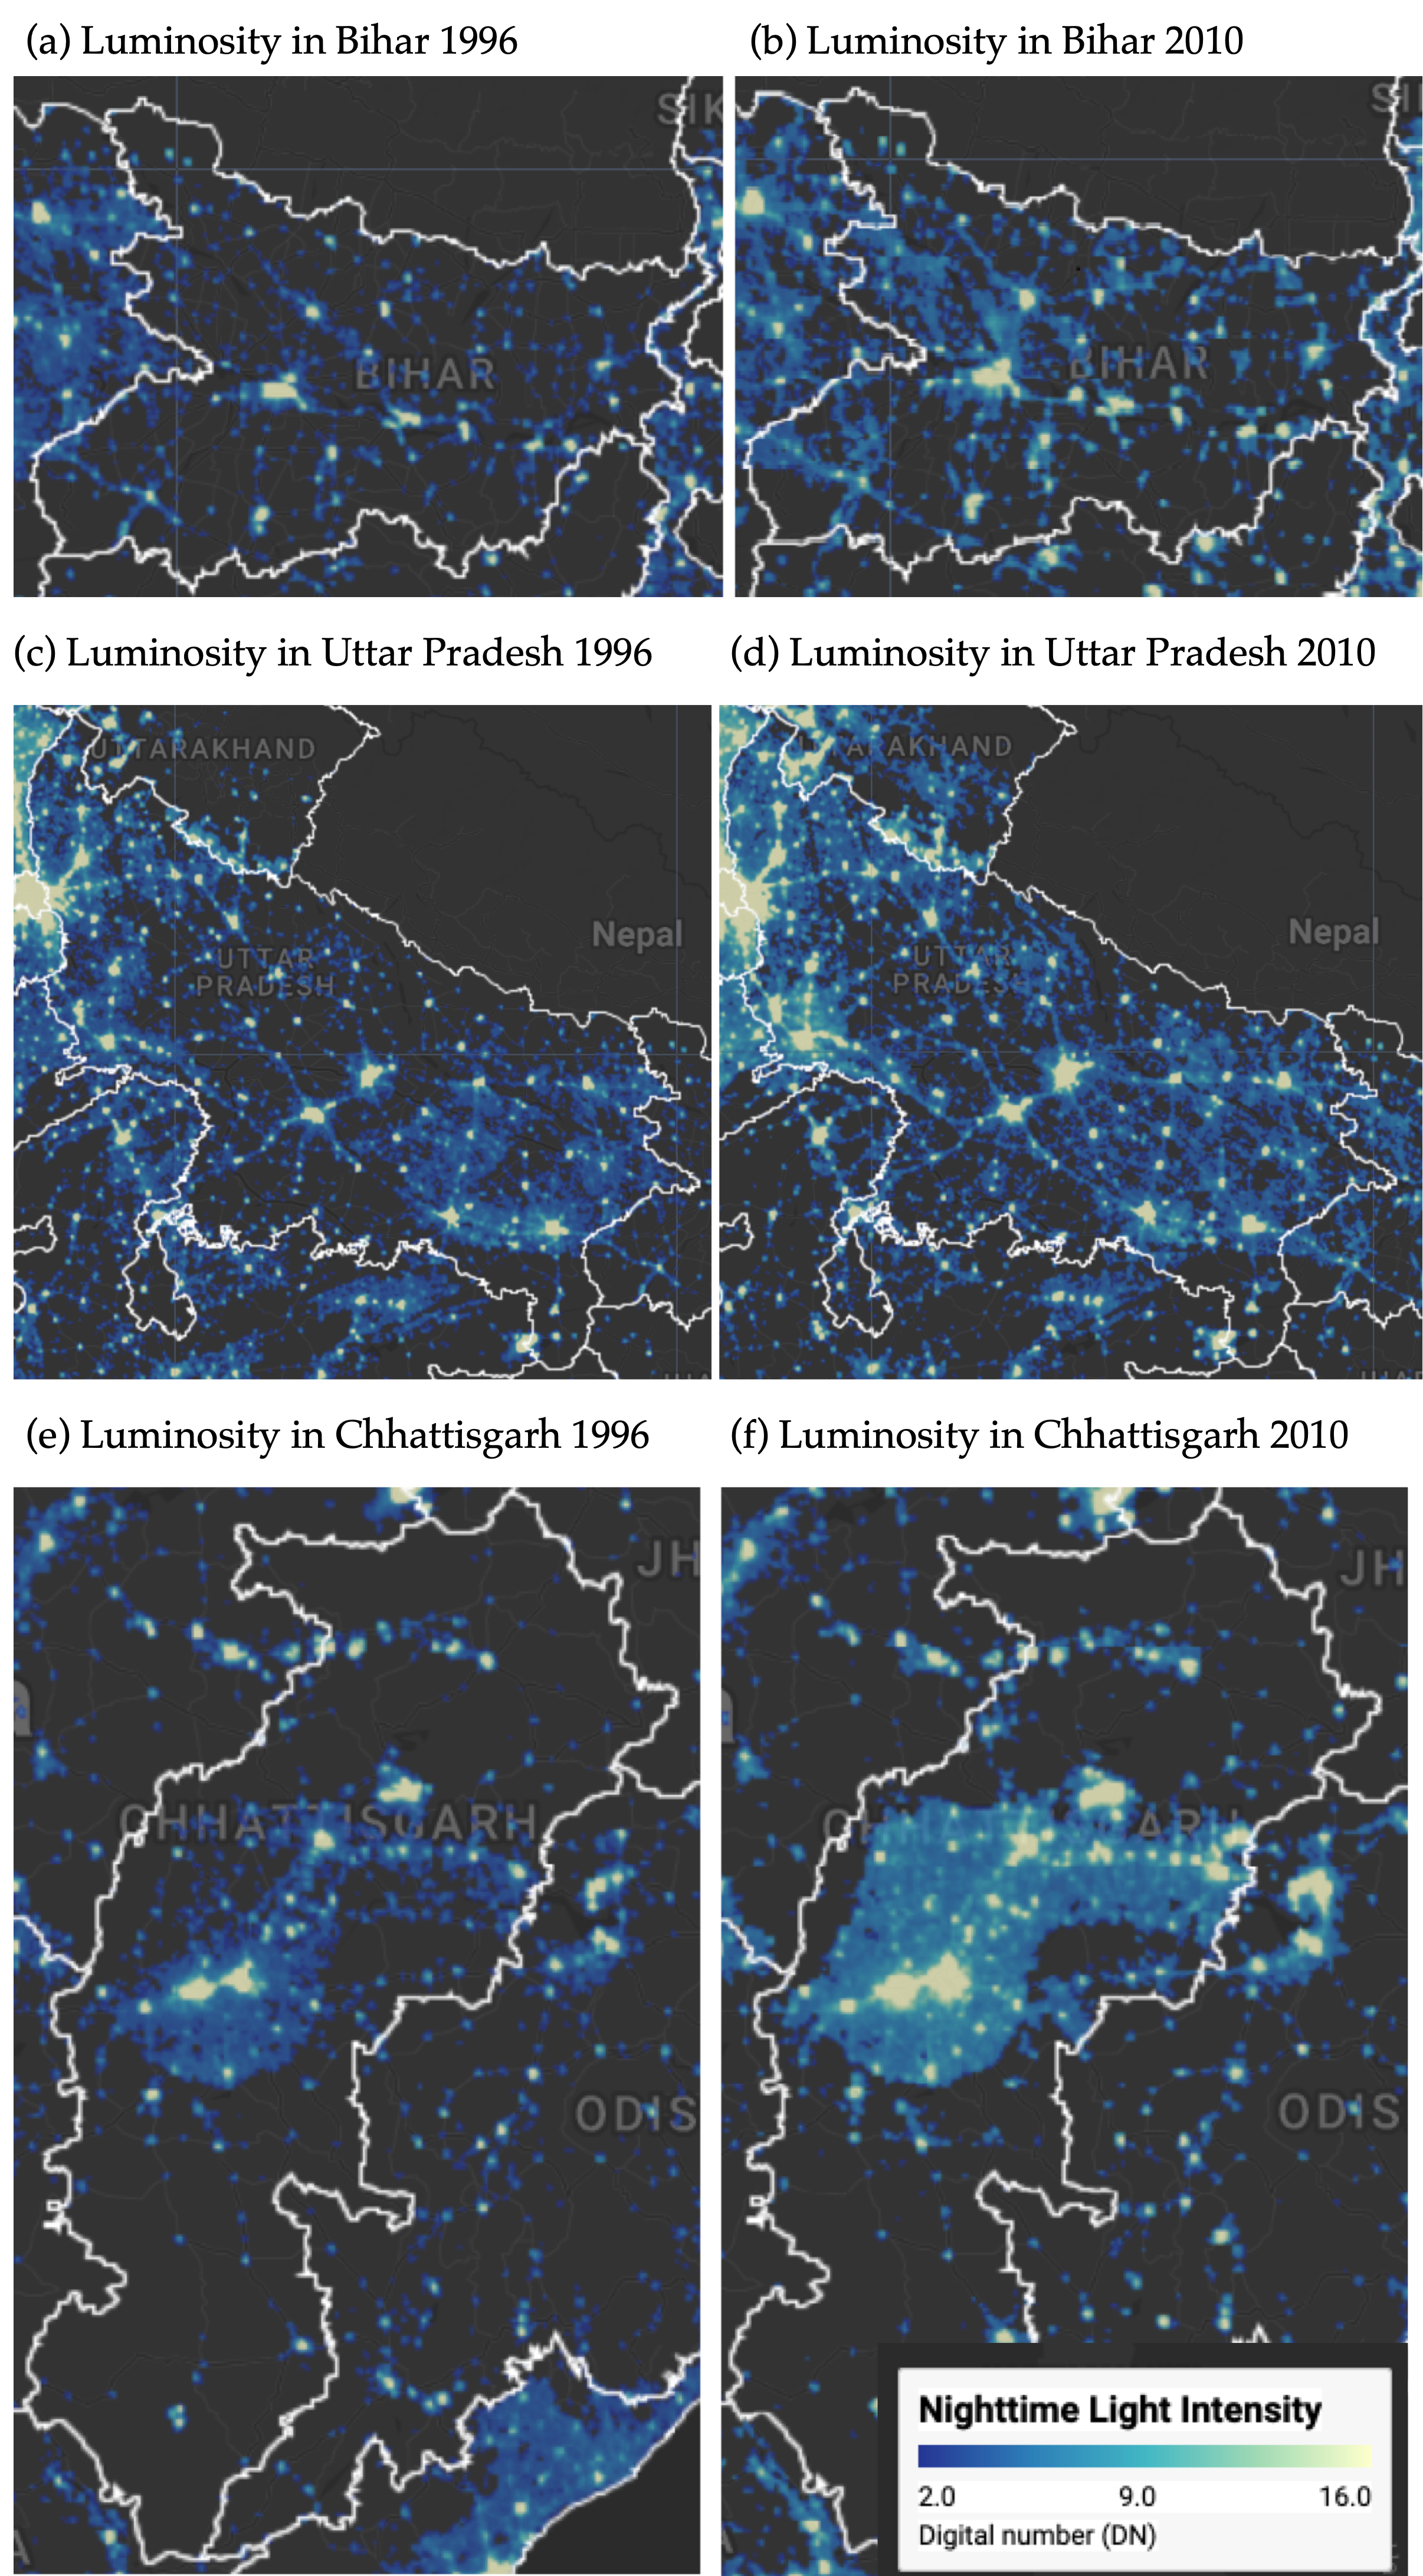
\includegraphics[width=0.75\linewidth,height=\textheight,keepaspectratio]{images/luminosity_map2.png}

}

\caption{\label{fig-map2}Some illustrative examples of regional
convergence Notes: The unit of measurement for Nighttime Light (NTL)
luminosity TBA. Interactive web application available at
https://bit.ly/india-rc-ntl . Source: Pre-processed luminosity images
are from the Earth Observation Group TBA.}

\end{figure}%

Next, we examine case studies of three economically disadvantaged states
in India to illustrate their growth patterns over the study period.
Among these, Bihar is the poorest, with a per capita income at 39.2\% of
the national average, while Uttar Pradesh and Chhattisgarh have per
capita incomes of 43.8\% and 52.3\% of the national average,
respectively.\footnote{The data is taken from a report by the Economic
  Advisory Council to the Prime Minister (EAC-PM), released on September
  18, 2024.} Figure 3 displays the change in luminosity in these three
states during our study period. Although these states remain among the
poorest, there is a noticeable increase in luminosity over the course of
the study.

\begin{figure}[H]

\centering{

\includegraphics[width=4.375in,height=4.375in]{index_files/figure-latex/notebooks-c02_regional_convergence_sc-fig-convergence-output-2.png}

}

\caption{\label{fig-convergence}Regional luminosity convergence across
districts in India Note: See Regional convergence notebook for source
code. Source: Data from Chanda and Kabiraj (2000).}

\end{figure}%

\textsubscript{Source:
\href{https://quarcs-lab.github.io/project2025s/notebooks/c02_regional_convergence_sc.ipynb.html\#cell-fig-convergence}{Regional
convergence}}

\subsection{Spatial dependence is a feature of the convergence
process}\label{spatial-dependence-is-a-feature-of-the-convergence-process}

In this study, the spatial lag terms of luminosity per capita growth and
initial luminosity per capita are computed by applying the Queen
contiguity weight matrix. FigureX visually presents the relationship
between local luminosity per capita growth rate and initial luminosity
per capita and its spatial lag term, respectively. The strong positive
spatial correlations observed between the variables and their
neighboring regions suggest that regional convergence is not an isolated
phenomenon, but rather a process intrinsically shaped by the influence
of adjacent regions. The Moran's I values of 0.644 and 0.739 for the
variables, coupled with a statistically significant spatial
autocorrelation in the error term, underscore the critical importance of
spatial dependence in convergence research. These findings demonstrate
that spatial interactions profoundly influence the convergence process,
rendering it imperative to incorporate spatial effects in empirical
analyses.

\begin{figure}[H]

\centering{

\pandocbounded{\includegraphics[keepaspectratio]{index_files/figure-latex/notebooks-c03_spatial_dependence_lisa-fig-wmatrix6nn-output-1.png}}

}

\caption{\label{fig-wmatrix6nn}Spatial connectivity structure based on
six nearest neighbors Note: See Spatial dependence notebook for source
code. Source: Data from Chanda and Kabiraj (2000).}

\end{figure}%

\textsubscript{Source:
\href{https://quarcs-lab.github.io/project2025s/notebooks/c03_spatial_dependence_lisa.ipynb.html\#cell-fig-Wmatrix6nn}{Spatial
dependence}}

This is a new figure.

\begin{figure}[H]

\centering{

\pandocbounded{\includegraphics[keepaspectratio]{index_files/figure-latex/notebooks-c03_spatial_dependence_lisa-fig-dependence-initial-output-1.png}}

}

\caption{\label{fig-dependence-initial}Spatial dependence in the initial
level of luminosity Note: See Regional convergence notebook for source
code. Source: Data from Chanda and Kabiraj (2000).}

\end{figure}%

\textsubscript{Source:
\href{https://quarcs-lab.github.io/project2025s/notebooks/c03_spatial_dependence_lisa.ipynb.html\#cell-fig-dependence-initial}{Spatial
dependence}}

This is another new figure.

\begin{figure}[H]

\centering{

\pandocbounded{\includegraphics[keepaspectratio]{index_files/figure-latex/notebooks-c03_spatial_dependence_lisa-fig-dependence-growth-output-1.png}}

}

\caption{\label{fig-dependence-growth}Spatial dependence in the growth
rate of luminosity Note: See Regional convergence notebook for source
code. Source: Data from Chanda and Kabiraj (2000).}

\end{figure}%

\textsubscript{Source:
\href{https://quarcs-lab.github.io/project2025s/notebooks/c03_spatial_dependence_lisa.ipynb.html\#cell-fig-dependence-growth}{Spatial
dependence}}

\subsection{Spatial spillovers accelerate regional
convergence}\label{spatial-spillovers-accelerate-regional-convergence}

The regression results of Table~\ref{tbl-models} provide evidence of
both unconditional and conditional convergence across districts in
India, with both conventional OLS and spatial econometric approaches
indicating significant negative relationships between initial luminosity
levels and subsequent growth rates. The direct effects, representing
within-district convergence, remain remarkably stable across
specifications, ranging from -0.020 to -0.026. This consistency across
different model specifications and estimation methods provides evidence
that poorer districts are indeed catching up to their wealthier
counterparts, even after controlling for various district
characteristics and state-level fixed effects.

\begin{longtable}[]{@{}
  >{\raggedright\arraybackslash}p{(\linewidth - 16\tabcolsep) * \real{0.1282}}
  >{\raggedright\arraybackslash}p{(\linewidth - 16\tabcolsep) * \real{0.1154}}
  >{\raggedright\arraybackslash}p{(\linewidth - 16\tabcolsep) * \real{0.0897}}
  >{\raggedright\arraybackslash}p{(\linewidth - 16\tabcolsep) * \real{0.1154}}
  >{\raggedright\arraybackslash}p{(\linewidth - 16\tabcolsep) * \real{0.1154}}
  >{\raggedright\arraybackslash}p{(\linewidth - 16\tabcolsep) * \real{0.1154}}
  >{\raggedright\arraybackslash}p{(\linewidth - 16\tabcolsep) * \real{0.0897}}
  >{\raggedright\arraybackslash}p{(\linewidth - 16\tabcolsep) * \real{0.1154}}
  >{\raggedright\arraybackslash}p{(\linewidth - 16\tabcolsep) * \real{0.1154}}@{}}
\caption{Unconditional and conditional convergence across
districts.}\label{tbl-models}\tabularnewline
\toprule\noalign{}
\begin{minipage}[b]{\linewidth}\raggedright
\end{minipage} & \begin{minipage}[b]{\linewidth}\raggedright
Model 1
\end{minipage} & \begin{minipage}[b]{\linewidth}\raggedright
\end{minipage} & \begin{minipage}[b]{\linewidth}\raggedright
Model 2
\end{minipage} & \begin{minipage}[b]{\linewidth}\raggedright
\end{minipage} & \begin{minipage}[b]{\linewidth}\raggedright
Model 3
\end{minipage} & \begin{minipage}[b]{\linewidth}\raggedright
\end{minipage} & \begin{minipage}[b]{\linewidth}\raggedright
Model 4
\end{minipage} & \begin{minipage}[b]{\linewidth}\raggedright
\end{minipage} \\
\midrule\noalign{}
\endfirsthead
\toprule\noalign{}
\begin{minipage}[b]{\linewidth}\raggedright
\end{minipage} & \begin{minipage}[b]{\linewidth}\raggedright
Model 1
\end{minipage} & \begin{minipage}[b]{\linewidth}\raggedright
\end{minipage} & \begin{minipage}[b]{\linewidth}\raggedright
Model 2
\end{minipage} & \begin{minipage}[b]{\linewidth}\raggedright
\end{minipage} & \begin{minipage}[b]{\linewidth}\raggedright
Model 3
\end{minipage} & \begin{minipage}[b]{\linewidth}\raggedright
\end{minipage} & \begin{minipage}[b]{\linewidth}\raggedright
Model 4
\end{minipage} & \begin{minipage}[b]{\linewidth}\raggedright
\end{minipage} \\
\midrule\noalign{}
\endhead
\bottomrule\noalign{}
\endlastfoot
& OLS & SDM & OLS & SDM & OLS & SDM & OLS & SDM \\
Direct & -0.020*** & -0.021*** & -0.022*** & -0.021*** & -0.025*** &
-0.026*** & -0.025*** & -0.025*** \\
& (0.002) & (0.002) & (0.003) & (0.002) & (0.003) & (0.002) & (0.003) &
(0.002) \\
Indirect & -- & -0.001 & -- & -0.001 & -- & -0.015* & -- & -0.012* \\
& & (0.006) & & (0.005) & & (0.008) & & (0.007) \\
Total & -0.020*** & -0.022*** & -0.022*** & -0.022*** & -0.025*** &
-0.041*** & -0.025*** & -0.037*** \\
& (0.002) & (0.006) & (0.003) & (0.005) & (0.003) & (0.008) & (0.003) &
(0.007) \\
Controls & No & No & No & No & Yes & Yes & Yes & Yes \\
State FE & No & No & Yes & Yes & No & No & Yes & Yes \\
AIC & -1945 & -2290 & -2413 & -2466 & -2211 & -2356 & -2469 & -2499 \\
\end{longtable}

Importantly, the spatial Durbin model uncovers significant spatial
spillover effects that are masked in traditional OLS estimations. These
indirect effects, which capture the influence of neighboring districts'
initial conditions on a district's growth rate, become increasingly
prominent and statistically significant as we add controls and state
fixed effects to our specifications. In our most comprehensive model, we
find a significant indirect effect of -0.012, suggesting that a
district's growth trajectory is meaningfully influenced by the initial
economic conditions of its neighbors. This finding highlights the
importance of geographical proximity and spatial interactions in the
convergence process.

The total impact of initial conditions on growth, combining both direct
and spillover effects, is substantially larger when we account for
spatial dependence. In our fully specified model, the total convergence
effect in the spatial Durbin model (-0.037) is approximately 48\% larger
than the OLS estimate (-0.025). This difference, supported by better
model fit statistics, indicates that conventional non-spatial approaches
may significantly underestimate the speed of regional convergence by
failing to capture the additional convergence channels created through
spatial spillovers. These results emphasize that regional convergence in
India operates not only through district-specific factors but also
through significant spatial interactions between neighboring districts.

\section{Discussion}\label{discussion}

\subsection{Better luminosity data from
VIIRS}\label{better-luminosity-data-from-viirs}

Our analysis, following Chanda and Kabiraj (2020), relies on
radiance-calibrated DMSP-OLS nighttime lights data covering the period
1996 to 2010. While this dataset has been widely validated as a proxy
for economic activity (Henderson, Storeygard, and Weil 2012; Chen and
Nordhaus 2011), DMSP-OLS data suffer from well-documented limitations
including top-coding in bright urban cores, lack of on-board calibration
leading to inter-satellite inconsistencies, and blooming artifacts that
spatially blur light sources beyond their true boundaries (Abrahams,
Oram, and Lozano-Gracia 2018). These measurement issues can attenuate
the precision of convergence estimates, particularly in rapidly
urbanizing districts where saturation may mask growth variation.

The Visible Infrared Imaging Radiometer Suite (VIIRS) Day/Night Band,
operational since 2012, represents a substantial improvement over
DMSP-OLS along multiple dimensions. VIIRS offers finer spatial
resolution (approximately 750 meters versus 2.7 kilometers), on-board
radiometric calibration that provides consistent quantitative
measurements, and a wider dynamic range that avoids saturation in urban
areas while detecting dim lights in rural settlements (Elvidge et al.
2017). Comparative evaluations have shown that VIIRS explains 10 to 15
percentage points more variation in subnational economic activity than
DMSP-OLS (Chen and Nordhaus 2015), and systematic assessments recommend
VIIRS as the preferred product for cross-sectional and recent
time-series studies (Gibson et al. 2021). Future extensions of our
convergence analysis using VIIRS data could yield more precise estimates
of both direct and indirect effects, particularly in districts where
DMSP saturation may have compressed the measured distribution of
luminosity.

A practical challenge for extending long-run convergence studies is the
discontinuity between DMSP (1992--2013) and VIIRS (2012--present) sensor
eras. Recent harmonization efforts, notably the global harmonized
nighttime light dataset by Li et al. (2020), have created consistent
27-year time series by calibrating VIIRS observations to DMSP-equivalent
units during the overlap period. Such harmonized datasets could enable
the extension of our spatial Durbin analysis to more recent periods,
allowing researchers to examine whether the convergence patterns and
spatial spillovers documented here have persisted, accelerated, or
changed in character as India's economy has continued to transform.

\subsection{New research directions}\label{new-research-directions}

While our analysis documents the average convergence effect and its
spatial spillover component, the cross-sectional regression framework
does not capture potential heterogeneity in convergence patterns across
the income distribution. Distribution dynamics approaches, as pioneered
by Quah (1996), could reveal whether Indian districts are converging to
a single steady state or forming distinct convergence clubs where
districts converge within groups but diverge across them. The regression
tree methods developed by Durlauf and Johnson (1995) for identifying
multiple growth regimes could be combined with spatial econometric
techniques (Rey and Montouri 1999) to examine whether geographic
clusters of districts follow distinct convergence trajectories,
potentially revealing spatial poverty traps or growth poles that are not
visible in average convergence estimates.

A second important direction concerns the causal identification of the
spillover channels that our spatial Durbin model captures in reduced
form. While our estimates document significant indirect effects, the
model does not identify whether these spillovers operate through
infrastructure linkages, labor migration, technology diffusion, or
market access channels. Quasi-experimental approaches, such as those
employed by Asher and Novosad (2020) to study the causal effects of
rural road construction on structural transformation in India, could be
embedded within spatial econometric frameworks to isolate specific
spillover mechanisms. Understanding which channels drive the indirect
convergence effects is critical for designing spatially targeted
policies that can amplify positive spillovers.

Third, the growing availability of diverse satellite products and
machine learning methods opens possibilities for richer measurement of
regional economic activity. Jean et al. (2016) demonstrated that
combining high-resolution daytime imagery with nighttime lights through
deep learning can substantially improve poverty prediction in
data-scarce settings. Similarly, Keola, Andersson, and Hall (2015)
showed that integrating nighttime lights with land cover data improves
economic measurement in agricultural areas where lights alone provide
weak signals. As Donaldson and Storeygard (2016) emphasize, the
expanding ecosystem of satellite-derived data---including vegetation
indices, built-up area detection, and high-frequency mobility
indicators---offers opportunities to construct multi-dimensional proxies
for regional economic activity that go beyond what nighttime lights
alone can capture.

\subsection{Research reproducibility and open
science}\label{research-reproducibility-and-open-science}

The complexity of satellite-based economic research---involving
multi-step data processing pipelines, spatial econometric estimation,
and geographic visualization---makes reproducibility both challenging
and essential. As Donaldson and Storeygard (2016) note, the processing
of satellite data requires careful documentation and sharing of code to
ensure that results can be replicated and extended. Each methodological
choice in the pipeline, from sensor inter-calibration to spatial weight
matrix construction, can affect empirical conclusions (Gibson et al.
2021), underscoring the need for transparent computational workflows
that allow other researchers to verify and build upon published
findings.

This article adopts a reproducible research approach through Quarto's
single-source publishing framework, where a single manuscript file
generates multiple output formats---interactive HTML, journal PDF, and
supplementary materials---from the same source. All computational
analyses are documented in embedded notebooks that readers can inspect
alongside the results they produce, creating a complete chain from raw
data to published findings. The interactive web-based visualization
tool, built on Google Earth Engine, allows researchers to independently
explore the spatial and temporal patterns in the nighttime light data,
facilitating verification of our visual findings and enabling new
discoveries beyond what static representations can convey.

Open-source tools and cloud computing platforms are rapidly lowering the
barriers to reproducible spatial economic research. Cloud-based
computational notebooks, such as those developed by Mendez and Patnaik
(2024) for processing nighttime lights data, eliminate the need for
specialized local software and provide accessible workflows for data
ingestion, preprocessing, spatial analysis, and visualization. The
combination of open data repositories, version-controlled code, and
cloud computing infrastructure creates an ecosystem where the full
analytical pipeline---from satellite imagery to econometric
results---can be made transparent, verifiable, and extensible by the
broader research community.

\section{Concluding remarks}\label{concluding-remarks}

This article examines regional convergence patterns across Indian
districts using satellite nighttime light data, interactive
visualizations, and spatial econometric modeling. Expanding on the work
of Chanda and Kabiraj (2020), we developed an interactive web-based
visualization tool that illustrates spatial and convergence patterns
across Indian districts. Spatial autocorrelation tests confirm that
spatial dependence is a fundamental characteristic of satellite data and
the regional convergence process in India. Estimates from our spatial
Durbin model indicate that incorporating spatial spillovers
significantly increases the estimated speed of regional convergence. The
total convergence effect in our fully specified model is approximately
36\% larger than conventional non-spatial estimates of Chanda and
Kabiraj (2020). This finding implies that non-spatial convergence models
may considerably underestimate the speed of regional convergence.
Additionally, it suggests that place-based development interventions may
have broader impacts, as their benefits can extend to neighboring
districts through spatial spillover effects.

These results have important implications for both research methodology
and policy design in developing countries. From a methodological
perspective, they highlight the value of combining new data sources,
interactive geospatial visualization tools, and spatial econometric
methods to better understand regional economic dynamics. From a policy
standpoint, they suggest that regional convergence operates not just
through district-specific factors, but through complex spatial
interactions that create additional channels for catch-up growth. This
spatial perspective is crucial for the analysis and design of policies
aimed at reducing regional inequalities in developing countries.

\section{Acknowledgments}\label{acknowledgments}

This work was supported by JSPS KAKENHI Grant Number 24K04884. During
the preparation of this work, the authors used Claude Code (Anthropic)
to assist with manuscript editing, computational notebook development,
and research infrastructure setup. After using this tool, the authors
reviewed and edited all content and take full responsibility for the
content of the publication.

\section{Conflict of Interest}\label{conflict-of-interest}

The authors declare no conflict of interest.

\section{Data and Code Availability}\label{data-and-code-availability}

All data and computational code used in this study are available in the
project repository: \url{https://github.com/quarcs-lab/project2025s}.
Also, the interactive HTML version of this manuscript
(\url{https://quarcs-lab.github.io/project2025s/}) embeds the
computational notebooks, allowing readers to inspect the complete
analytical pipeline from raw data to published results.

\phantomsection\label{refs}
\begin{CSLReferences}{1}{0}
\bibitem[\citeproctext]{ref-abrahams_etal_deblurring}
Abrahams, Alexei, Christopher Oram, and Nancy Lozano-Gracia. 2018.
{``Deblurring DMSP Nighttime Lights: A New Method Using Gaussian Filters
and Frequencies of Illumination.''} \emph{Remote Sensing of Environment}
210: 242--58. \url{https://doi.org/10.1016/j.rse.2018.03.018}.

\bibitem[\citeproctext]{ref-adhikari_dhital_decentralization}
Adhikari, Bibek, and Ramesh Dhital. 2020. {``Decentralization and
Regional Convergence: Evidence from Nighttime Lights.''} \emph{Journal
of Development Economics} 145: 102467.
\url{https://doi.org/10.1016/j.jdeveco.2020.102467}.

\bibitem[\citeproctext]{ref-asher_novosad_rural_roads}
Asher, Sam, and Paul Novosad. 2020. {``Rural Roads and Local Economic
Development.''} \emph{American Economic Review} 110 (3): 797--823.
\url{https://doi.org/10.1257/aer.20180268}.

\bibitem[\citeproctext]{ref-beyer_jain_sinha_covid}
Beyer, Robert C. M., Tarun Jain, and Biswa N. Sinha. 2021. {``Lights
Out? COVID-19 Containment Policies and Economic Activity.''}
\emph{Journal of Asian Economics} 74: 101318.
\url{https://doi.org/10.1016/j.asieco.2021.101318}.

\bibitem[\citeproctext]{ref-chakravarty_dehejia_gst}
Chakravarty, Shankha, and Rajeev Dehejia. 2019. {``The GST and Regional
Divergence in India: A Nightlights Perspective.''} \emph{Economic and
Political Weekly} 54 (42): 47--54.

\bibitem[\citeproctext]{ref-chanda_cook_demonetization}
Chanda, Areendam, and Justin Cook. 2022. {``Demonetization and Its
Redistributive Effects: Evidence from India.''} \emph{Journal of
Development Economics} 156: 102835.
\url{https://doi.org/10.1016/j.jdeveco.2022.102835}.

\bibitem[\citeproctext]{ref-chanda_kabiraj_district_convergence}
Chanda, Areendam, and Shankha Kabiraj. 2020. {``Shedding Light on
Regional Growth and Convergence in India.''} \emph{World Development}
133: 104961. \url{https://doi.org/10.1016/j.worlddev.2020.104961}.

\bibitem[\citeproctext]{ref-chen_nordhaus_luminosity_gdp}
Chen, Xi, and William D. Nordhaus. 2011. {``Using Luminosity Data as a
Proxy for Economic Statistics.''} \emph{Proceedings of the National
Academy of Sciences} 108 (21): 8589--94.
\url{https://doi.org/10.1073/pnas.1017031108}.

\bibitem[\citeproctext]{ref-chen_nordhaus_measurement_error}
---------. 2015. {``A Test of the New VIIRS Lights Data Set: Population
and Economic Output in Africa.''} \emph{Remote Sensing} 7 (4): 4937--47.
\url{https://doi.org/10.3390/rs70404937}.

\bibitem[\citeproctext]{ref-cook_shah_nregs}
Cook, Justin, and Manisha Shah. 2022. {``Aggregate Effects from Public
Works: Evidence from India.''} \emph{Review of Economics and Statistics}
104 (2): 201--17. \url{https://doi.org/10.1162/rest_a_00951}.

\bibitem[\citeproctext]{ref-donaldson_storeygard_remotesensing}
Donaldson, Dave, and Adam Storeygard. 2016. {``The View from Above:
Applications of Satellite Data in Economics.''} \emph{Journal of
Economic Perspectives} 30 (4): 171--98.
\url{https://doi.org/10.1257/jep.30.4.171}.

\bibitem[\citeproctext]{ref-durlauf_johnson_convergence_clubs}
Durlauf, Steven N., and Paul A. Johnson. 1995. {``Multiple Regimes and
Cross-Country Growth Behaviour.''} \emph{Journal of Applied
Econometrics} 10 (4): 365--84.
\url{https://doi.org/10.1002/jae.3950100404}.

\bibitem[\citeproctext]{ref-elvidge_etal_viirs}
Elvidge, Christopher D., Kimberly E. Baugh, Mikhail Zhizhin, Feng-Chi
Hsu, and Tilottama Ghosh. 2017. {``VIIRS Night-Time Lights.''}
\emph{International Journal of Remote Sensing} 38 (21): 5860--79.
\url{https://doi.org/10.1080/01431161.2017.1342050}.

\bibitem[\citeproctext]{ref-ertur_koch_spatial_growth}
Ertur, Cem, and Wilfried Koch. 2007. {``Growth, Technological
Interdependence and Spatial Externalities: Theory and Evidence.''}
\emph{Journal of Applied Econometrics} 22 (6): 1033--62.
\url{https://doi.org/10.1002/jae.963}.

\bibitem[\citeproctext]{ref-fischer_spatial_mrw}
Fischer, Manfred M. 2011. {``A Spatial Mankiw-Romer-Weil Model: Theory
and Evidence.''} \emph{Annals of Regional Science} 47 (2): 419--36.
\url{https://doi.org/10.1007/s00168-010-0384-6}.

\bibitem[\citeproctext]{ref-gennaioli_etal_growth_regions}
Gennaioli, Nicola, Rafael La Porta, Florencio Lopez-de-Silanes, and
Andrei Shleifer. 2014. {``Growth in Regions.''} \emph{Journal of
Economic Growth} 19 (3): 259--309.
\url{https://doi.org/10.1007/s10887-014-9105-9}.

\bibitem[\citeproctext]{ref-gibson_etal_ntl_measurement}
Gibson, John, Susan Olivia, Geua Boe-Gibson, and Chao Li. 2021. {``Which
Night Lights Data Should We Use in Economics, and Where?''}
\emph{Journal of Development Economics} 149: 102602.
\url{https://doi.org/10.1016/j.jdeveco.2020.102602}.

\bibitem[\citeproctext]{ref-henderson_storeygard_weil_lights}
Henderson, J. Vernon, Adam Storeygard, and David N. Weil. 2012.
{``Measuring Economic Growth from Outer Space.''} \emph{American
Economic Review} 102 (2): 994--1028.
\url{https://doi.org/10.1257/aer.102.2.994}.

\bibitem[\citeproctext]{ref-jean_etal_poverty_prediction}
Jean, Neal, Marshall Burke, Michael Xie, W. Matthew Davis, David B.
Lobell, and Stefano Ermon. 2016. {``Combining Satellite Imagery and
Machine Learning to Predict Poverty.''} \emph{Science} 353 (6301):
790--94. \url{https://doi.org/10.1126/science.aaf7894}.

\bibitem[\citeproctext]{ref-jha_talathi_colonial_india}
Jha, Saumitra, and Anand Talathi. 2021. {``Colonial Institutions and
Long-Run Development in India: Evidence from Nightlights.''}
\emph{Journal of Development Economics} 153: 102726.
\url{https://doi.org/10.1016/j.jdeveco.2021.102726}.

\bibitem[\citeproctext]{ref-keola_etal_lights_poverty}
Keola, Souknilanh, Magnus Andersson, and Ola Hall. 2015. {``Monitoring
Economic Development from Space: Using Nighttime Light and Land Cover
Data to Measure Economic Growth.''} \emph{World Development} 66:
322--34. \url{https://doi.org/10.1016/j.worlddev.2014.08.017}.

\bibitem[\citeproctext]{ref-lessmann_seidel_regional_inequality}
Lessmann, Christian, and André Seidel. 2017. {``Regional Inequality,
Convergence, and Its Determinants: A View from Outer Space.''}
\emph{European Economic Review} 92: 110--32.
\url{https://doi.org/10.1016/j.euroecorev.2016.11.009}.

\bibitem[\citeproctext]{ref-li_etal_harmonization}
Li, Xi, Yuyu Zhou, Min Zhao, and Xia Zhao. 2020. {``A Harmonized Global
Nighttime Light Dataset 1992--2018.''} \emph{Scientific Data} 7 (1):
168. \url{https://doi.org/10.1038/s41597-020-0510-y}.

\bibitem[\citeproctext]{ref-mendez_patnaik_notebook}
Mendez, Carlos, and Ayush Patnaik. 2024. {``A Python Notebook for
Processing Nighttime Lights Data: Methods and Applications.''} GitHub
Repository. \url{https://github.com/quarcs-lab/project2022p}.

\bibitem[\citeproctext]{ref-pinkovskiy_salaimartin_lights_poverty}
Pinkovskiy, Maxim, and Xavier Sala-i-Martin. 2016. {``Lights, Camera,
Income! Illuminating the National Accounts-Household Surveys Debate.''}
\emph{Quarterly Journal of Economics} 131 (2): 579--631.
\url{https://doi.org/10.1093/qje/qjw003}.

\bibitem[\citeproctext]{ref-quah_twin_peaks}
Quah, Danny T. 1996. {``Twin Peaks: Growth and Convergence in Models of
Distribution Dynamics.''} \emph{Economic Journal} 106 (437): 1045--55.
\url{https://doi.org/10.2307/2235377}.

\bibitem[\citeproctext]{ref-rey_spatial_dynamics}
Rey, Sergio J., and Brett D. Montouri. 1999. {``US Regional Income
Convergence: A Spatial Econometric Perspective.''} \emph{Regional
Studies} 33 (2): 143--56.
\url{https://doi.org/10.1080/00343409950122945}.

\end{CSLReferences}




\end{document}
